%%%%%%%%%%%%%%%%%%%%%%%%%%%%%%%%%%%%%%%%%%%%%%%%%%%%%%%%%%%%%%%%%%%%%%%%%%
%%%%%%%%%%%%   CAPTER 2   %%%%%%%%%%%%%%%%%%%%%%%%%%%%%%%%%%%%%%%%%%%%%%%%
%%%%%%%%%%%%%%%%%%%%%%%%%%%%%%%%%%%%%%%%%%%%%%%%%%%%%%%%%%%%%%%%%%%%%%%%%%
\chapter{Background and Related Work}
\label{chap:related_work}
%
Collecting data on user behavior or equipment is a delicate task. On the one hand there are legal hurdles like
the European Unions General Data Protection Regulation (GDPR), on the other hand is the users trust
in a software project. If a project looses the trust of users, it may face with a massive loss in
user. This can lead to a drop in revenue for commercial projects and a major setback for any open source
project. If a project violates the GDPR it can be considerably fined and take significant damage from it.\\

Never the less, collecting data is important to evolve and improve a software project. Usage data can help
to shape a project in a way, that it attracts more user, or increases it's security and reliability.
It can help to identify no longer, or intensely used components, which can help to improve maintenance
processes.\\ 

%%% TODO: eine Seite füllen %%%


Therefore many projects collect data on there users. In section \ref{sec:related_work:related_sw} we are
going to discuss techniques used by different projects. Furthermore related research on anonymization of user data 
(section \ref{sec:related_work:data_aononymization}) and it's transmission (section \ref{sec:related:data_transmission}) will be presented


%%%%%%%%%%%%%%%%%%%%%%%%%%%%%%%%%%%%%
%%%%%%%%%%%%%%%%%%%%%%%%%%%%%%%%%%%%%
%%%%%%%%%%%%   SECTION   %%%%%%%%%%%%
%%%%%%%%%%%%%%%%%%%%%%%%%%%%%%%%%%%%%
%%%%%%%%%%%%%%%%%%%%%%%%%%%%%%%%%%%%%
\section{Data Anonymization}
\label{sec:related_work:data_aononymization}
%
%% privacy
%% differential privacy

%
%%%%%%%%%%%%%%%%%%%%%%%%%%%%%%%%%%%%%
%%%%%%%%%%%% Subsection %%%%%%%%%%%%%
%%%%%%%%%%%%%%%%%%%%%%%%%%%%%%%%%%%%%
%
\subsection{Law Regulations}
\label{subsec:related:law}
Anonymity is defined by DIN EN ISO/IEC 29100 as an information characteristic, that does not allow to identify a person directly or indirectly\cite{noauthor_din_2020}. It furthermore declares anonymization as a process, in which personally identifiable information (PII) is irrevocable transformed. This transformation denies the ability for an entity to identify a person indirectly or directly by itself or in cooperation with another entity.\\

A major advantage for anonymized data is the exclusion of the GDPR legislation. Recital 26 of the regulation excludes anonymized data explicitly.\\ 
"The principles of data protection should therefore not apply to anonymous information, namely information which does not relate to an identified or identifiable natural person or to personal data rendered anonymous in such a manner that the data subject is not or no longer identifiable. This Regulation does not therefore concern the processing of such anonymous information, including for statistical or research purposes."\cite{european_union_regulation_2016}

%
%%%%%%%%%%%%%%%%%%%%%%%%%%%%%%%%%%%%%
%%%%%%%%%%%% Subsection %%%%%%%%%%%%%
%%%%%%%%%%%%%%%%%%%%%%%%%%%%%%%%%%%%%
%
\subsection{\textit{k}-anonymity}
\label{subsec:related:kanon}

%%%%%%%%%%%%%%%%%%%%%%%%%%%%%%%%%%%%%
%%%%%%%%%%%%%%%%%%%%%%%%%%%%%%%%%%%%%
%%%%%%%%%%%%   SECTION   %%%%%%%%%%%%
%%%%%%%%%%%%%%%%%%%%%%%%%%%%%%%%%%%%%
%%%%%%%%%%%%%%%%%%%%%%%%%%%%%%%%%%%%%
\section{Data Transmission}
\label{sec:related:data_transmission}
%
The Tor Project is probably the most known approach for anonymized data transmission over the Internet. Besides Tor we are going to discuss different approaches to transmit data over a network. In \ref{subsec:related:overlay} the Tor and I2P overlay network are going to be discussed, followed by systems used by current browser. Finally in \ref{subsec:related:protocols} we discuss different protocols available for data transmission.


%
%%%%%%%%%%%%%%%%%%%%%%%%%%%%%%%%%%%%%
%%%%%%%%%%%% Subsection %%%%%%%%%%%%%
%%%%%%%%%%%%%%%%%%%%%%%%%%%%%%%%%%%%%
%
%%%% Overlay Networks
%
\subsection{Overlay Networks}
\label{subsec:related:overlay}
%
%%% Tor %%%
\subsubsection{Tor}

%%% I2P %%%
\subsubsection{I2P}

%%%%%%%%%%%%%%%%%%%%%%%%%%%%%%%%%%%%%
%%%%%%%%%%%% Subsection %%%%%%%%%%%%%
%%%%%%%%%%%%%%%%%%%%%%%%%%%%%%%%%%%%%
%
%%%% Special systems
%
\subsection{Special Systems}
\label{subsec:related:special}
%
%%% Prio
\subsubsection{Prio}
    Prio was developed by Corrigan-Gibbs et al.\cite{corrigan-gibbs_prio_2017} in 2017 as a privacy-preserving
    system for collecting aggregated statistics
    
    Prio\cite{corrigan-gibbs_prio_2017}, which was developed at Stanford University's Computer Science department for nonsensitive data already covered by their Telemetry tool. 
    Prio splits the collected client data into shares. 
    The parts are send to different servers and aggregated with shares of other users before being published (see figure \ref{fig:prio_overview})\cite{corrigan-gibbs_prio_2017}.\\
    Prio promises privacy, as long as one of the servers is honest, therefore providing strong cryptographic privacy. A limited form of robustness is provided as long as all server are honest. It can detect and discard syntactically incorrect client data while preserving the privacy of the data. However, Prio can not prevent a client from sending in range data, that is untrue\cite{corrigan-gibbs_prio_2017}.\\
    Prio is in experimental use by Firefox Origin Telemetry\\
    
    \begin{figure}
        \centering
        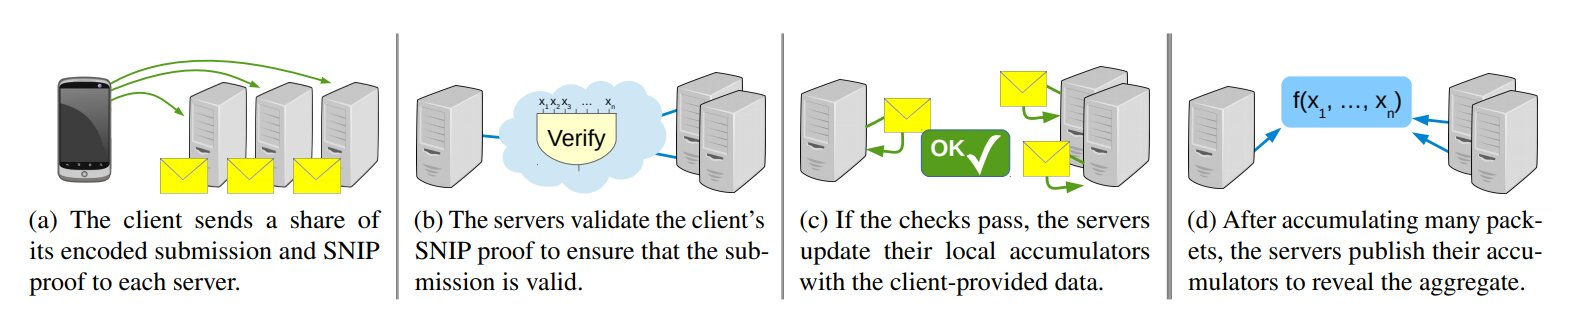
\includegraphics[width=\textwidth]{latex/figures/prio_overview.jpg}
        \caption{Overview of Prios processing pipeline\cite{corrigan-gibbs_prio_2017}}
        \label{fig:prio_overview}
    \end{figure}

%%% Prochlo %%%
\subsubsection{Prochlo}
    Prochlo describes a system architecture for large-scale monitoring of software usage activities. The system uses an "Encode, Shuffle, Analyze" approach. Thereby data is encoded and encrypted on one side. It's also the encoders objective to add noise and take care of the randomness of the collected data\cite{bittau_prochlo_2017}.\\
    Afterwards the data is transmitted to a centralized shuffler. They are responsible for the masking of the data origin by removing metadata (IP address, order and time of arrival).
    The data is held for a prolonged time and transmitted only, when a single data item is hidden in a crowd of similar data items. Therefore shufflers need to be trusted entities and separated from the analyzer\cite{bittau_prochlo_2017}. To add further trustworthiness they should be run by third party. The aggregated and reordered data is send out at random intervals to further increase the decoupling of time of arrival and enhance the privacy of clients.\\
    After transmission the data is decrypted, stored and aggregated by the analyzer. 
    Added noise and fragmentation on the encoder site, as well as shuffling may be sufficient to provide differential anonymity in this system.
    
    Prochlo is developed by Google and used by Chrome, as well as, in modified from, by Brave.

%%%%%%%%%%%%%%%%%%%%%%%%%%%%%%%%%%%%%
%%%%%%%%%%%% Subsection %%%%%%%%%%%%%
%%%%%%%%%%%%%%%%%%%%%%%%%%%%%%%%%%%%%
%
%%%% Protocols and Tools
%
\subsection{Protocols}
\label{subsec:related:protocols}
%

%%% Other Protocols and Tools
\subsubsection{Other Protocols and Tools}


%%% DNS 
\subsection{Domain Name System - DNS}



%%%%%%%%%%%%%%%%%%%%%%%%%%%%%%%%%%%%%
%%%%%%%%%%%%%%%%%%%%%%%%%%%%%%%%%%%%%
%%%%%%%%%%%%   SECTION   %%%%%%%%%%%%
%%%%%%%%%%%%%%%%%%%%%%%%%%%%%%%%%%%%%
%%%%%%%%%%%%%%%%%%%%%%%%%%%%%%%%%%%%%
\section{Data Robustness}
\label{sec:related:data_robustness}


%%%%%%%%%%%%%%%%%%%%%%%%%%%%%%%%%%%%%
%%%%%%%%%%%% Subsection %%%%%%%%%%%%%
%%%%%%%%%%%%%%%%%%%%%%%%%%%%%%%%%%%%%
%
%%%% SNIP
%
\subsection{Secret-Shared Non-Interactive Proof - SNIP}
\label{subsec:related:snip}
%


%%%%%%%%%%%%%%%%%%%%%%%%%%%%%%%%%%%%%
%%%%%%%%%%%% Subsection %%%%%%%%%%%%%
%%%%%%%%%%%%%%%%%%%%%%%%%%%%%%%%%%%%%
%
%%%% NIZK
%
\subsection{Non-Interactive Zero-Knowledge Proof - NIZK}
\label{subsec:related:nizk}
%


%%%%%%%%%%%%%%%%%%%%%%%%%%%%%%%%%%%%%
%%%%%%%%%%%% Subsection %%%%%%%%%%%%%
%%%%%%%%%%%%%%%%%%%%%%%%%%%%%%%%%%%%%
%
%%%% SNARK
%
\subsection{Succinct Non-Interactive Arguments of Knowledge - SNARK}
\label{subsec:snark}
%




%%%%%%%%%%%%%%%%%%%%%%%%%%%%%%%%%%%%%
%%%%%%%%%%%%%%%%%%%%%%%%%%%%%%%%%%%%%
%%%%%%%%%%%%   SECTION   %%%%%%%%%%%%
%%%%%%%%%%%%%%%%%%%%%%%%%%%%%%%%%%%%%
%%%%%%%%%%%%%%%%%%%%%%%%%%%%%%%%%%%%%
\section{Related Software}
\label{sec:related_work:related_sw}
%

%%% Ubuntu %%%
\subsection{Ubuntu}

%%% KDE %%%
\subsection{KDE}


\newpage
%%% Firefox %%%
\subsection{Firefox}
    By default Firefox collects a wide range of data. These data collections are called Pings. Each Ping contains a certain type of information. At the time of writing there are at least 27 different Ping types in use\cite{mozilla_telemetry_nodate}.
    The "main" Ping is used for most telemetric data. It contains extensive health and performance information on Firefox, but also most system information. The JSON structure of a "main" Ping can be seen in Mozillas pipeline schema GitHub repository \cite{mozilla_mozilla-servicesmozilla-pipeline-schemas_2020}. 
    Besides information on CPU, GPU and operating system it contains information on installed add-ons and the reason for sending the Ping.
    It is send at least every 24 hours, but also on startup and other occasions. While basic telemetry, like the main ping can be disabled on the Settings page, Firefox will still send selected Pings to it's server, unless disabled in \textit{about:config}.
    %TODO: verify with wireshark
    To send the collected Telemetry, Firefox uses a program called Ping Sender.
    This will send a HTTP POST to the Edge Server where it is forwarded to the data pipeline if it's is formatted correctly.
    If a client IP address is available at the decoder, the geolocation will be determined and saved.
    The IP address gets discarded from the data set in the process. \cite{mozilla_overview_2020},\cite{mozilla_http_2020},\cite{firefox_ping_nodate}.\\
    A reduced data pipeline can be seen in figure \ref{fig:moz_data_flow}.
    
    
    \begin{wrapfigure}{R}{0.4\textwidth}
        \centering
        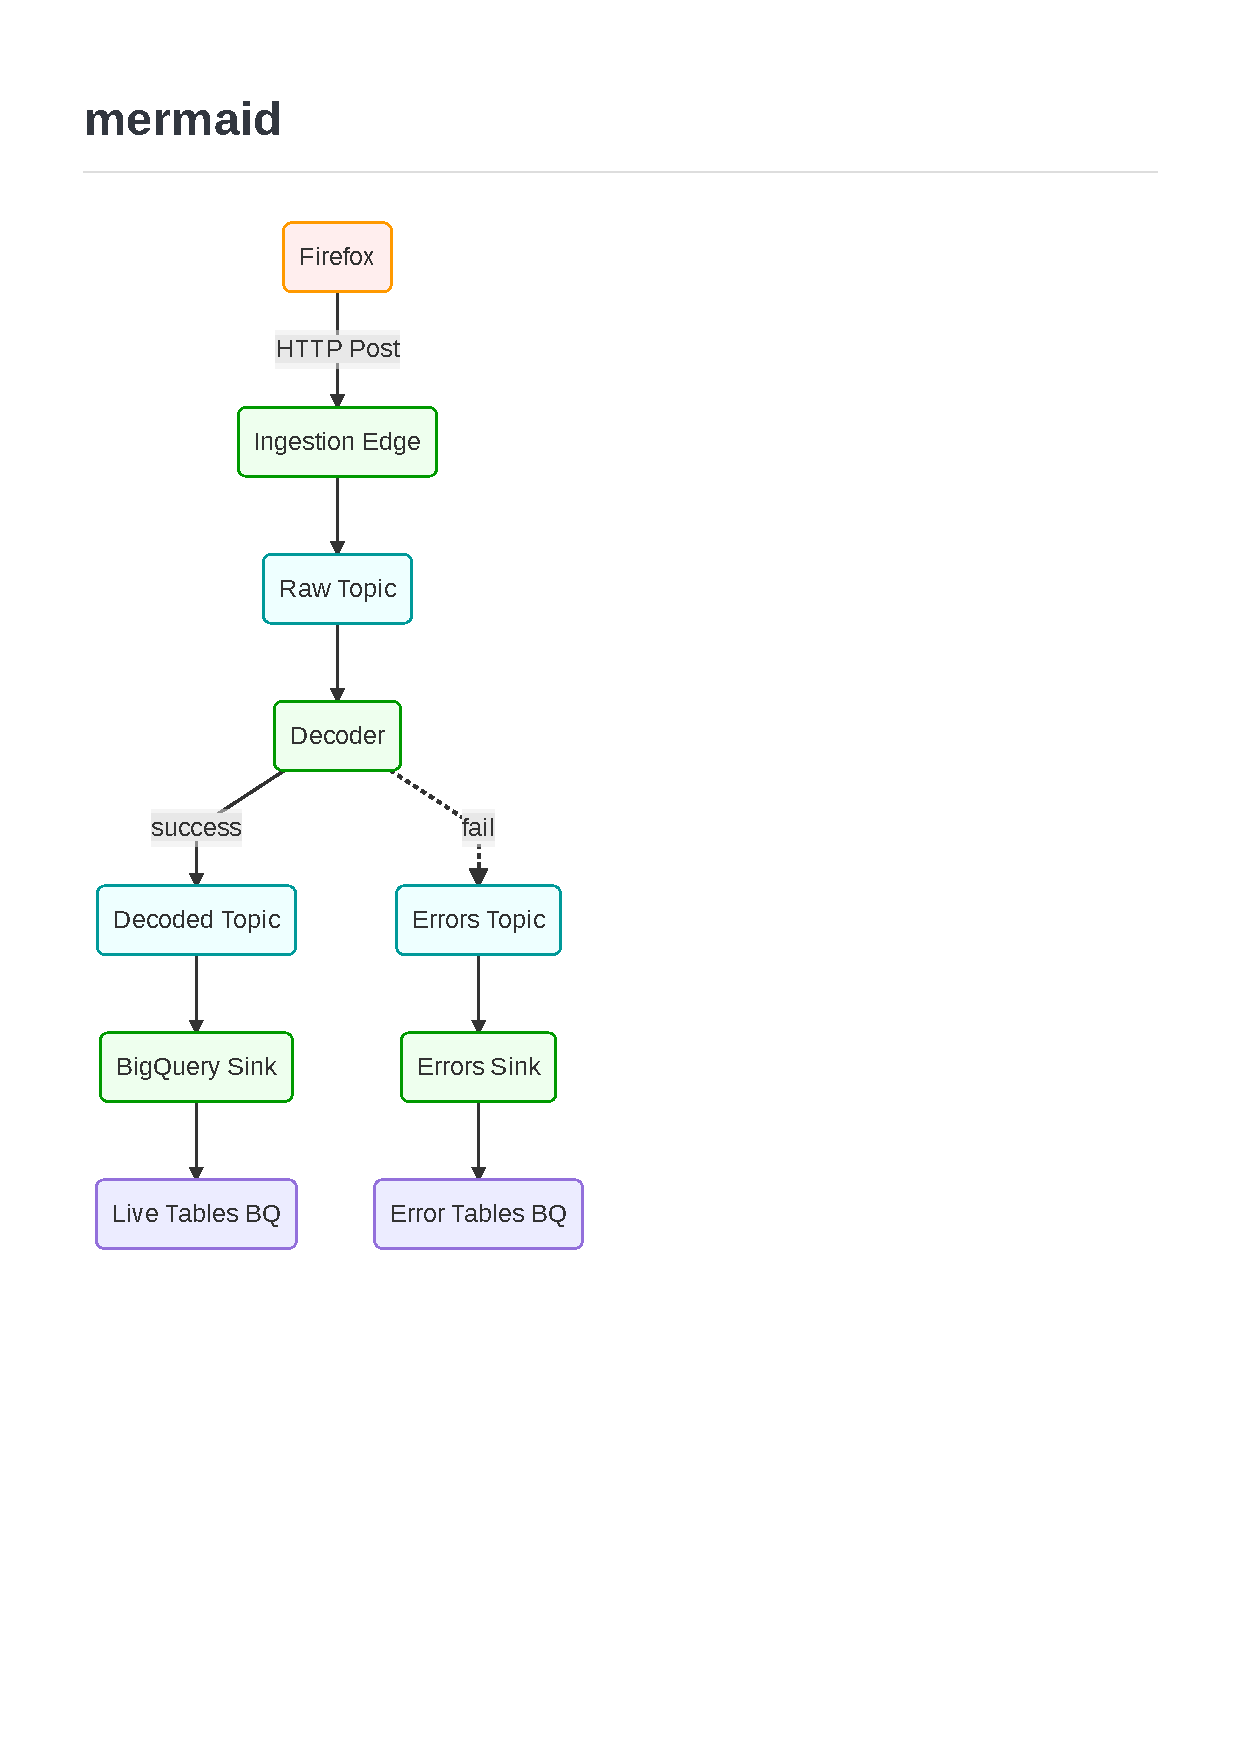
\includegraphics[clip, trim=0.5cm 8cm 8cm 3.5cm, width=0.5\textwidth]{latex/figures/firefox_telemetry_graph}
        \caption{Firefox data flow based on \cite{mozilla_overview_2020}}
        \label{fig:moz_data_flow}
    \end{wrapfigure}

    Mozilla was experimenting with Prio in 2018 \cite{helmer_testing_2018} and based on the experiment they developed Firefox Origin Telemetry\cite{englehardt_next_2019} which is, at the time of writing, in use only for content blocking and still experimental\cite{noauthor_origin_nodate}.\\


%%% Brave %%%
\subsection{Brave}
    Brave uses a technique called Privacy Preserving Product Analytics (P3A) for telemetry data, which can be turned off at any time.
    They claim, that their P3A does cover way more, than expected by GDPR. No personally identifiable data (PII) is collected or transmitted.\\
    Therefore Braves telemetry process is split into two phases.\\
    The first phase consists of several multiple choice questions, for which the answer is send individually.
    Each question poses a number of answers. Quantifiable questions, like the the number of open tabs, provide ranges for each answer for enhanced privacy\cite{brave_privacy-preserving_2019}. These Questions and possible answers can be reviewed in Braves GitHub repository\cite{brave_software_inc_brave-browser_2019}.
    The questions of phase one can be seen in Listing \ref{list:brave_question} in the appendix as well.\\
    At a randomized time after opening the browser, the number of open tabs is counted and send out once an hour with further information\cite{brave_privacy-preserving_2019}.
    An answer contains:
    \begin{itemize}
        \item Question number, Answer number
        \item OS/Plattform
        \item Release information (nightly/dev/bet/release)
        \item Week of installation (if installation was within 90 days)
        \item Country (if fewer than 6000 installs per week this is removed)
        \item Referral code (only if within 90 days of install and referrer is big enough)
    \end{itemize}
    Every answer is send to Braves content delivery network (CDN) and stripped of the IP address of the client at the edge of the CDN\cite{brave_privacy-preserving_2019}.
    . 
    The Second Phase uses a protocol based on Prochlo(see \ref{sec:related_work:data_transmission}. 
    
    
    
    The study Leith conducted in February 2020 \cite{leith_web_2020} supports Brave Software Inc. claims
    for a privacy caring browser.\\
    In his survey Leigh evaluated the privacy settings of six browsers (Brave, Chrome, Edge, Firefox, Safari and Yandex) has been compared. While Brave and Firefox (with changed defaults) where strongly focused on privacy all Browser did send there reports in combination with the users IP address\cite{leith_web_2020}.
    This is problematic, as an IP address can be used to pin down the users geolocation\cite{koch_geolocation_2013}. Workplaces or homes can be derived based on the time people spend in places during day or night. 
    While Brave Software Inc. claims, that they remove the IP address at the edge of their CDN, the user has to trust the CDN operator to strip the send data of the address for phase one answers. In Phase two the user has to trust the shuffler to remove the meta data from the collected data. 

%%%%%%%%%%%%%%%%%%%%%%%%%%%%%%%%%%%%%
%%%%%%%%%%%%%%%%%%%%%%%%%%%%%%%%%%%%%
%%%%%%%%%%%%   SECTION   %%%%%%%%%%%%
%%%%%%%%%%%%%%%%%%%%%%%%%%%%%%%%%%%%%
%%%%%%%%%%%%%%%%%%%%%%%%%%%%%%%%%%%%%
\section{Summary}
In this chapter we summarised previous work on related topics. This allows us to narrow our research.
Therefor we concentrate our research on <technology> as we want to achieve.
%


  